\documentclass{beamer}

\usepackage{amsmath}
\usepackage{amssymb}
\usepackage{graphicx}


\begin{document}
%============================================================================= %
\begin{frame}
	
\frametitle{Review of Differentiation}
\begin{figure}
\centering
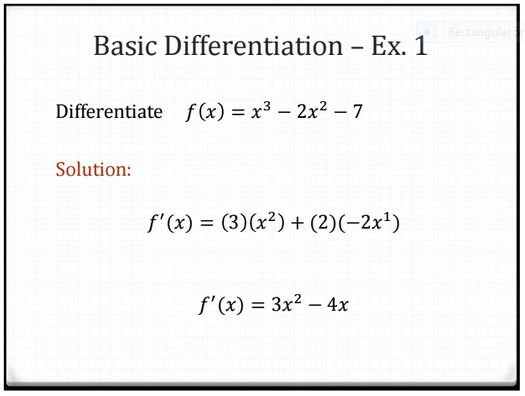
\includegraphics[width=0.95\linewidth]{diff1a}

\end{figure}
\end{frame}
%============================================================================= %
\begin{frame}
	
	\frametitle{Review of Differentiation}
	
\end{frame}
%============================================================================= %
\begin{frame}
	
	\frametitle{Review of Differentiation}
	\begin{figure}
		\centering
		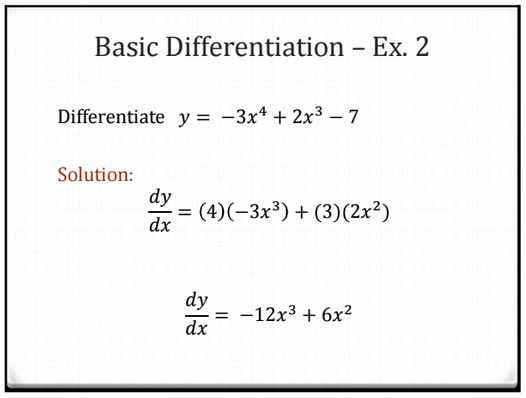
\includegraphics[width=0.95\linewidth]{diff1b}
		
	\end{figure}
\end{frame}
%============================================================================= %
\begin{frame}
	
	\frametitle{Review of Differentiation}
	
\end{frame}
%============================================================================= %
\begin{frame}
	
	\frametitle{Review of Differentiation}
	\begin{figure}
		\centering
		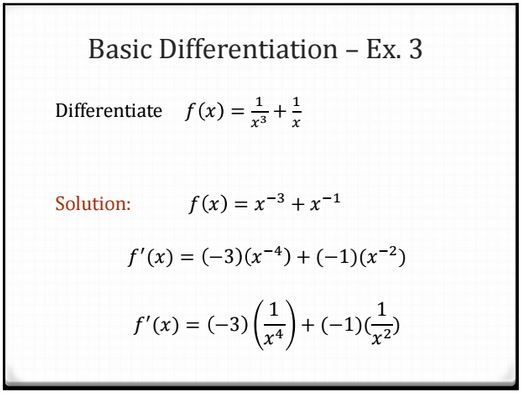
\includegraphics[width=0.95\linewidth]{diff1c}
		
	\end{figure}
\end{frame}
%============================================================================= %
\begin{frame}
	
	\frametitle{Review of Differentiation}
	
\end{frame}
%============================================================================= %
\begin{frame}
	
	\frametitle{Review of Differentiation}
	\begin{figure}
		\centering
		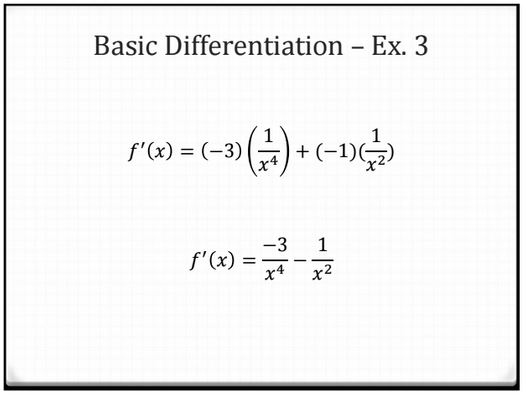
\includegraphics[width=0.95\linewidth]{diff1d}
		
	\end{figure}
\end{frame}
%============================================================================= %
\begin{frame}
	
	\frametitle{Review of Differentiation}
	
\end{frame}
%============================================================================= %
\begin{frame}
	
	\frametitle{Review of Differentiation}
	\begin{figure}
		\centering
		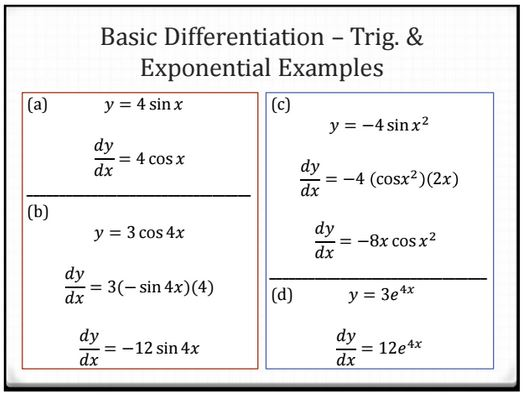
\includegraphics[width=0.95\linewidth]{diff1e}
		
	\end{figure}
\end{frame}
%============================================================================= %
\begin{frame}
	
	\frametitle{Review of Differentiation}
	
\end{frame}
%============================================================================= %

\begin{frame}
	
	\frametitle{Review of Differentiation}
	
\end{frame}
%============================================================================= %
\end{document}
\begin{description}
%% PART 5. 

\item[5a] Find partial derivatives of functions of two variables as well as higher partial derivatives; 
\item[5b] apply to analysis of small errors.
\end{description}

